\documentclass[12pt, a4paper]{article}

% ── Encodage & langue ──────────────────────────────────────────────────────────
\usepackage[utf8]{inputenc}
\usepackage[T1]{fontenc}
\usepackage[french]{babel}

% ── Mise en page ───────────────────────────────────────────────────────────────
\usepackage[top=2.2cm, bottom=2.2cm, left=2.5cm, right=2.5cm]{geometry}
\usepackage{parskip}
\setlength{\parskip}{6pt}

% ── Typographie ────────────────────────────────────────────────────────────────
\usepackage{lmodern}
\usepackage{microtype}
\usepackage{eurosym}

% ── Couleurs & graphiques ──────────────────────────────────────────────────────
\usepackage[dvipsnames]{xcolor}
\usepackage{graphicx}
\usepackage{float}
\usepackage{subcaption}

% ── Tableaux ───────────────────────────────────────────────────────────────────
\usepackage{booktabs}
\usepackage{array}

% ── Liens ──────────────────────────────────────────────────────────────────────
\usepackage[hidelinks]{hyperref}

% ── En-tête / pied de page ────────────────────────────────────────────────────
\usepackage{fancyhdr}
\pagestyle{fancy}
\fancyhf{}
\rhead{\small Projet Cloud - M2SDD}
\lhead{\small Analyse Black Friday avec Azure}
\lfoot{Matthieu PELINGRE}
\rfoot{\thepage}
\renewcommand{\headrulewidth}{0.4pt}

% ── Affichage du code et url ─────────────────────────────────────────────────────
\definecolor{colortt}{HTML}{0b8509}
\newcommand{\mytexttt}[1]{\texttt{\textbf{\textcolor{colortt}{#1}}}}
\newcommand{\bhref}[2]{\textcolor{blue}{\href{#1}{#2}}}

% ── Couleur titre section ─────────────────────────────────────────────────────
\usepackage{titlesec}
\definecolor{azureblue}{RGB}{0, 120, 212}
\titleformat{\section}{\large\bfseries\color{azureblue}}{}{0em}{}[\titlerule]
\titleformat{\subsection}{\normalsize\bfseries\color{azureblue!80}}{}{0em}{}

% ── Boîtes d'observation ──────────────────────────────────────────────────────
\usepackage{tcolorbox}
\tcbuselibrary{skins, breakable}
\newtcolorbox{observation}{
  colback=azureblue!5,
  colframe=azureblue!60,
  fonttitle=\bfseries\small,
  title=Observation,
  boxrule=0.5pt,
  arc=3pt,
  left=4pt, right=4pt, top=3pt, bottom=3pt,
  breakable
}

% ──────────────────────────────────────────────────────────────────────────────
\begin{document}

% ── Page de titre ─────────────────────────────────────────────────────────────
\begin{titlepage}
  \centering
  \vspace*{2cm}
  {\Huge\bfseries\color{azureblue}
    Analyse des comportements d'achat\\[0.4em]
    sur le dataset Black Friday\\[0.4em]
    avec Microsoft Azure\par}
  \vspace{1.5cm}
  {\large Matthieu PELINGRE\par}
  \vspace{2cm}
  \rule{0.5\textwidth}{0.4pt}\\[1em]
  {\large Master 2 Science des Données - M2SDD\\
  Cours de Cloud Computing\par}
  \vspace{1cm}
  {\large Mars 2026\par}
  \vspace{2cm}
  \begin{tabular}{ll}
    \textbf{Dataset} & Black Friday Sales (Kaggle, 550\,068 transactions) \\[4pt]
    \textbf{Services Azure} & Blob Storage, Azure OpenAI, Text Analytics \\[4pt]
    \textbf{Visualisation} & Power BI \\
  \end{tabular}
\end{titlepage}

% ──────────────────────────────────────────────────────────────────────────────
\section{Introduction et architecture du pipeline}

Ce projet s'inscrit dans le cadre du cours de Cloud du Master 2 Science des Données. L'objectif est de construire un pipeline complet, de la collecte jusqu'à la visualisation, en s'appuyant sur des services \textbf{Microsoft Azure}.

Le jeu de données choisi est le \textit{Black Friday Sales Dataset}, disponible sur Kaggle, qui regroupe \textbf{550\,068 transactions} effectuées lors d'un Black Friday par 5\,891 clients distincts sur 3\,631 produits. Le dataset étant purement transactionnel et encodé, une étape d'enrichissement par IA a été ajoutée pour tirer parti des services Azure d'intelligence artificielle.

\medskip
\textbf{Pipeline mis en œuvre :}

\begin{center}
\begin{tabular}{ccccc}
  \textbf{Kaggle} & $\longrightarrow$ & \textbf{Azure Blob Storage} &
  $\longrightarrow$ & \textbf{Azure OpenAI} \\
  & & & & $\downarrow$ \\
  \textbf{Power BI} & $\longleftarrow$ & \textbf{Blob Storage (résultats)} &
  $\longleftarrow$ & \textbf{Azure Text Analytics} \\
\end{tabular}
\end{center}

% ──────────────────────────────────────────────────────────────────────────────
\section{Exploration et ingestion des données}

\subsection{Description du dataset}

Le dataset contient 12 variables :

\begin{center}
\begin{tabular}{lll}
  \toprule
  \textbf{Variable} & \textbf{Type} & \textbf{Description} \\
  \midrule
  \mytexttt{User\_ID} & Catégoriel & Identifiant client \\
  \mytexttt{Product\_ID} & Catégoriel & Identifiant produit \\
  \mytexttt{Gender} & Catégoriel & Sexe (F / M) \\
  \mytexttt{Age} & Catégoriel & Tranche d'âge (7 modalités) \\
  \mytexttt{Occupation} & Catégoriel encodé & Profession (21 codes anonymes) \\
  \mytexttt{City\_Category} & Catégoriel & Catégorie de ville (A, B, C) \\
  \mytexttt{Stay\_In\_Current\_City\_Years} & Catégoriel & Ancienneté dans la ville \\
  \mytexttt{Marital\_Status} & Binaire & Statut marital \\
  \mytexttt{Product\_Category\_1/2/3} & Catégoriel encodé & Catégories produit \\
  \mytexttt{Purchase} & Numérique & Montant d'achat (devise non précisée) \\
  \bottomrule
\end{tabular}
\end{center}

\begin{observation}
La quasi-totalité des variables numériques sont en réalité des variables catégorielles encodées. De plus, la devise associée à \mytexttt{Purchase} n'est pas précisée dans le dataset, nous supposons qu'il s'agit de roupies indiennes (ce qui serait cohérent avec les montants observés et les données démographiques).
\end{observation}

\subsection{Valeurs manquantes et nettoyage}

Les valeurs manquantes se concentrent sur les catégories secondaires et tertiaires des produits, qui sont optionnelles :

\begin{itemize}
  \item \mytexttt{Product\_Category\_2} : 31,6~\% de valeurs manquantes
  \item \mytexttt{Product\_Category\_3} : 69,7~\% de valeurs manquantes
\end{itemize}

Ces valeurs ont été remplacées par \mytexttt{0} (catégorie inexistante), les catégories valides étant encodées entre 1 et 20.

\subsection{Principales observations exploratoires}

Quelques indicateurs clés issus de l'EDA :

\begin{itemize}
  \item \textbf{75~\% des transactions} sont effectuées par des hommes
  \item Le groupe d'âge le plus actif est \textbf{26--35 ans} (219\,587 transactions, soit 40~\% du total), cohérent avec une tranche à la fois plus nombreuse et à fort pouvoir d'achat
  \item Le \textbf{panier moyen} est de \textbf{9\,264 unités monétaires} (médiane : 8\,047), avec un écart-type de 5\,023 révélant une forte disparité
  \item Les \textbf{catégories 5, 1 et 8} sont les plus achetées en volume, tandis que les \textbf{catégories 9, 10 et 16} affichent les montants moyens les plus élevés
  \item Les villes de \textbf{catégorie C} concentrent proportionnellement plus de gros montants que les catégories A et B
\end{itemize}

\begin{observation}
Le segment \textbf{Homme / 26--35 ans} domine si fortement (40~\% des transactions) qu'il écrase les autres profils dans toutes les analyses par catégorie. Cette surreprésentation est à prendre en compte dans toute modélisation ou segmentation ultérieure.
\end{observation}

\subsection{Ingestion dans Azure Blob Storage}

Après nettoyage et encodage des variables catégorielles, le fichier
\mytexttt{blackfriday\_clean.csv} (22,75~Mo, 550\,068 lignes) a été téléversé
dans un conteneur Azure Blob Storage privé.

\begin{figure}[H]
  \centering
  \begin{subfigure}[b]{0.38\textwidth}
    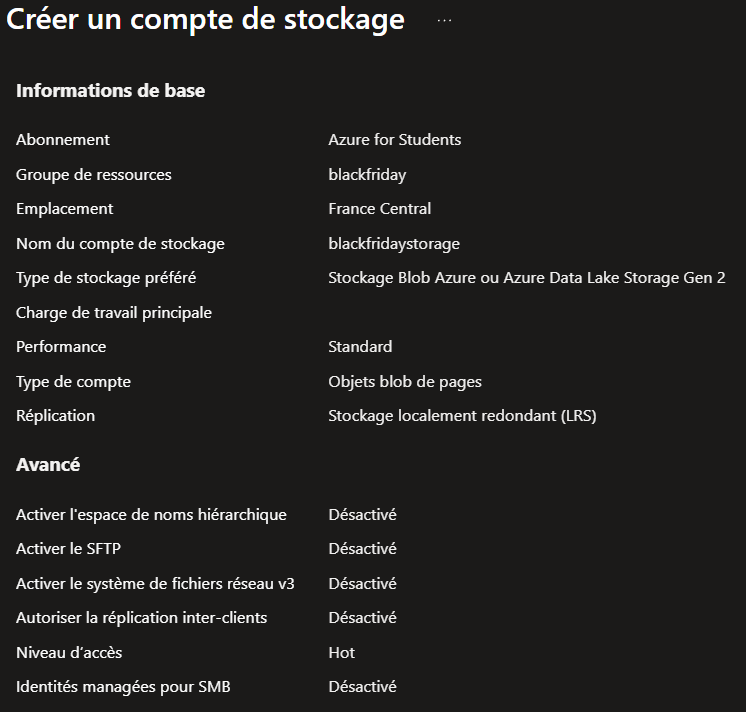
\includegraphics[width=\textwidth]{../pictures/1-ingestion/1.5-compte_stockage3.png}
    \caption{Compte de stockage}
  \end{subfigure}
  \hfill
  \begin{subfigure}[b]{0.60\textwidth}
    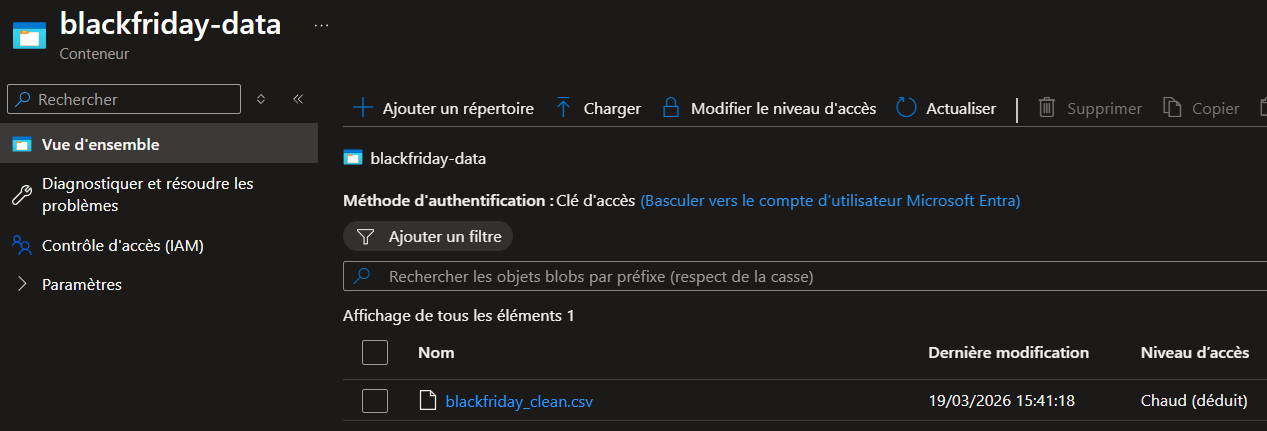
\includegraphics[width=\textwidth]{../pictures/1-ingestion/1.10-televersement.png}
    \caption{Fichier téléversé dans le conteneur Blob}
  \end{subfigure}
  \caption{Configuration Azure Blob Storage et téléversement du dataset}
\end{figure}

La configuration retenue est : compte de stockage \textit{Standard}, redondance \textit{LRS} (Locally Redundant Storage), niveau d'accès \textit{Chaud (Hot)}. La vérification post-téléversement a confirmé l'intégrité du fichier (22,75~Mo, 550\,068 lignes, 12 colonnes).

% ──────────────────────────────────────────────────────────────────────────────
\section{Enrichissement par les services IA d'Azure}

Le dataset Black Friday étant purement transactionnel, il ne contient aucune donnée textuelle. Nous avons contourné cette limite en générant des \textbf{avis clients synthétiques} pour alimenter les services d'analyse d'Azure.

\subsection{Segmentation et construction de personas (Azure OpenAI)}

Pour limiter les coûts API, nous avons travaillé sur des \textbf{données agrégées} : 14 segments (croisement Sexe $\times$ Tranche d'âge) résumant l'ensemble du dataset. Pour chaque segment, le modèle \textbf{GPT-4o mini} (déployé via Azure AI Foundry) a généré :

\begin{enumerate}
  \item Des \textbf{descriptions pour les 20 catégories de produits} anonymes (ex. : catégorie 1 = \og Électronique de luxe \fg{}, catégorie 8 = \og Chaussures tendance \fg{})
  \item Des \textbf{personas marketing} pour chaque segment (profil fictif mais crédible)
  \item Des \textbf{avis clients fictifs} (5 catégories $\times$ 3 niveaux de notation = 15 avis)
\end{enumerate}

\begin{figure}[H]
  \centering
  \begin{subfigure}[b]{0.43\textwidth}
    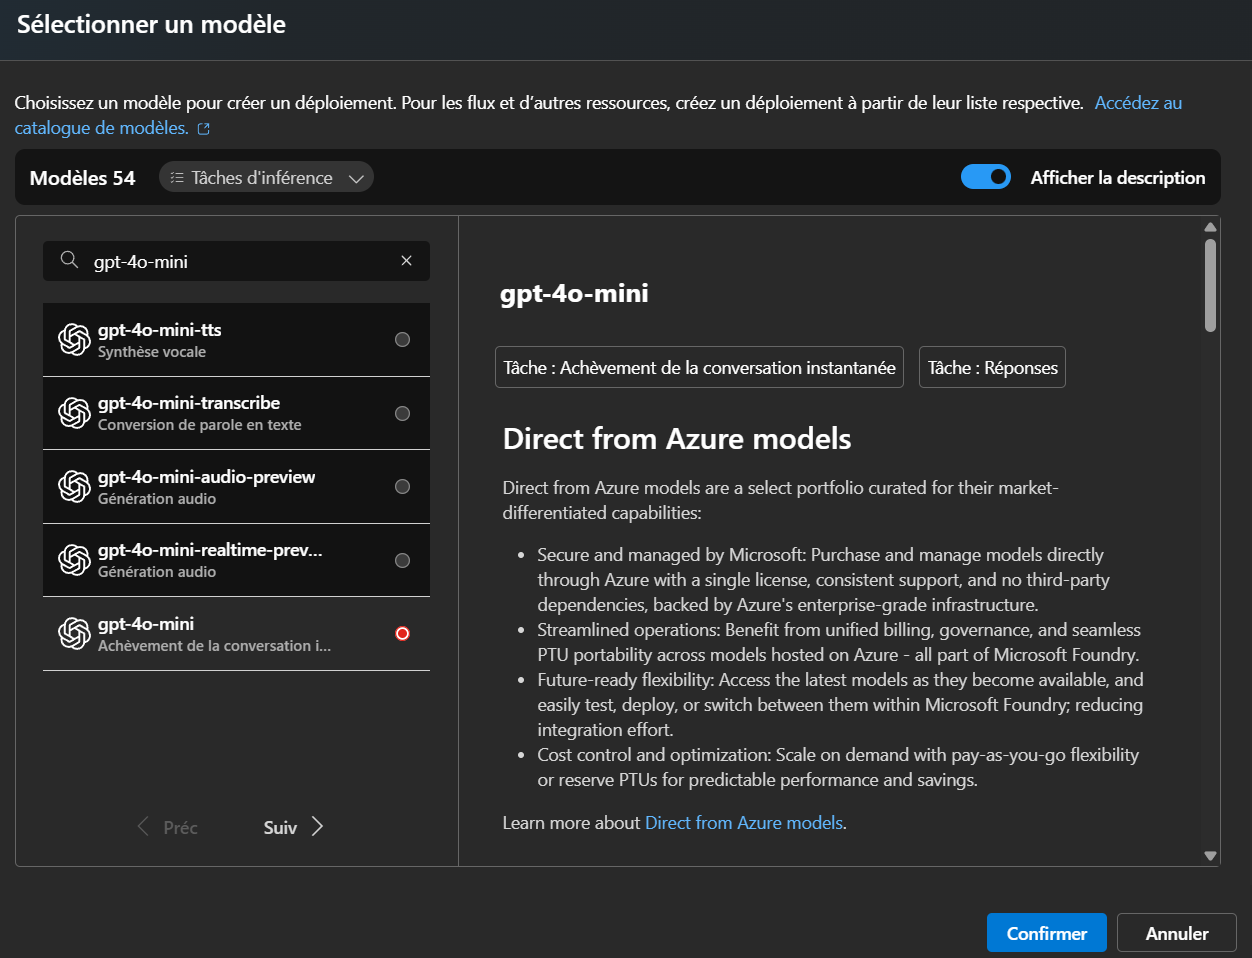
\includegraphics[width=\textwidth]{../pictures/2-azure_ai/2.3-azure_openai4.png}
    \caption{Déploiement GPT-4o mini}
  \end{subfigure}
  \hfill
  \begin{subfigure}[b]{0.55\textwidth}
    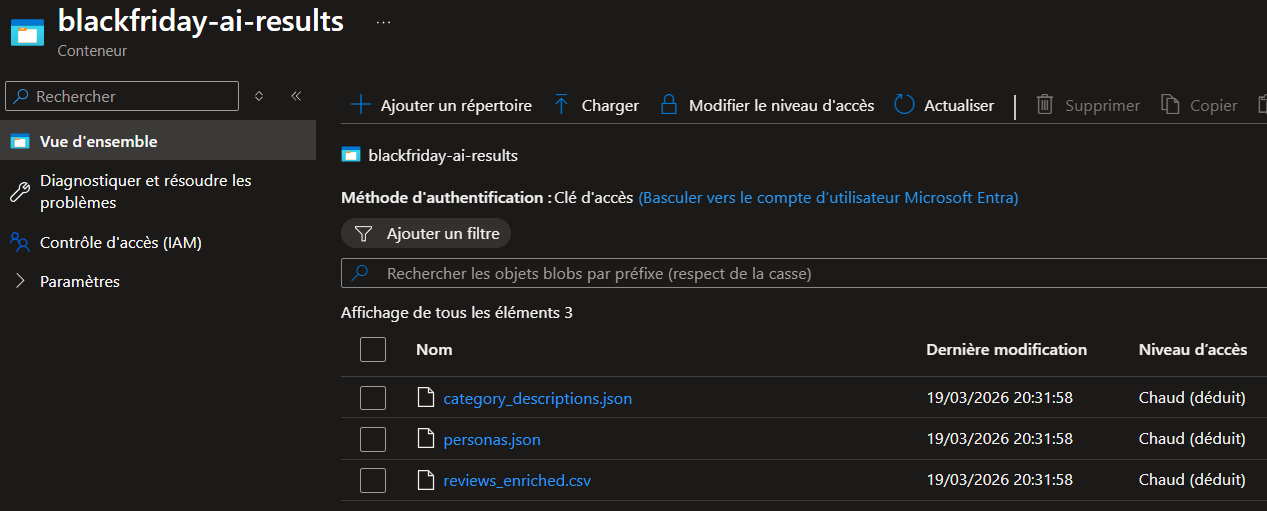
\includegraphics[width=\textwidth]{../pictures/2-azure_ai/2.9-export.png}
    \caption{Export des résultats vers Blob Storage}
  \end{subfigure}
  \caption{Azure OpenAI : génération de contenu et export}
\end{figure}

\begin{observation}
Le persona dominant dans les avis est \og Lucas, 30 ans \fg{} (segment H/26--35), reflet direct de la sur-représentation de ce groupe dans le dataset. La génération de personas par LLM constitue un \textbf{cas d'usage marketing classique} : enrichir une segmentation RFM (Récence, Fréquence, Montant) avec des profils narratifs directement actionnables par des équipes communication.
\end{observation}

\subsection{Analyse de sentiment et extraction de mots-clés (Azure Text Analytics)}

Les 15 avis générés ont ensuite été soumis au service \textbf{Azure Language / Text Analytics} pour :

\begin{itemize}
  \item \textbf{Analyse de sentiment} : classification positif / négatif / neutre avec score de confiance (13 analyses réussies sur 15, soit 87~\%)
  \item \textbf{Extraction de mots-clés} (key phrases) : identification des thèmes récurrents par catégorie de produit
\end{itemize}

Exemples de mots-clés extraits par catégorie :

\begin{center}
\begin{tabular}{ll}
  \toprule
  \textbf{Catégorie} & \textbf{Mots-clés dominants} \\
  \midrule
  Électronique de luxe & luxe, appareil photo, smartphone, passionnés \\
  Accessoires de mode & qualité, montre, élégante, compliments \\
  Chaussures tendance & chaussures, confort, prix, journées \\
  Articles de maison & qualité, décoration, produits, maison \\
  Vêtements décontractés & tissu, t-shirt, collection, qualité \\
  \bottomrule
\end{tabular}
\end{center}

\begin{figure}[H]
  \centering
  \begin{subfigure}[b]{0.38\textwidth}
    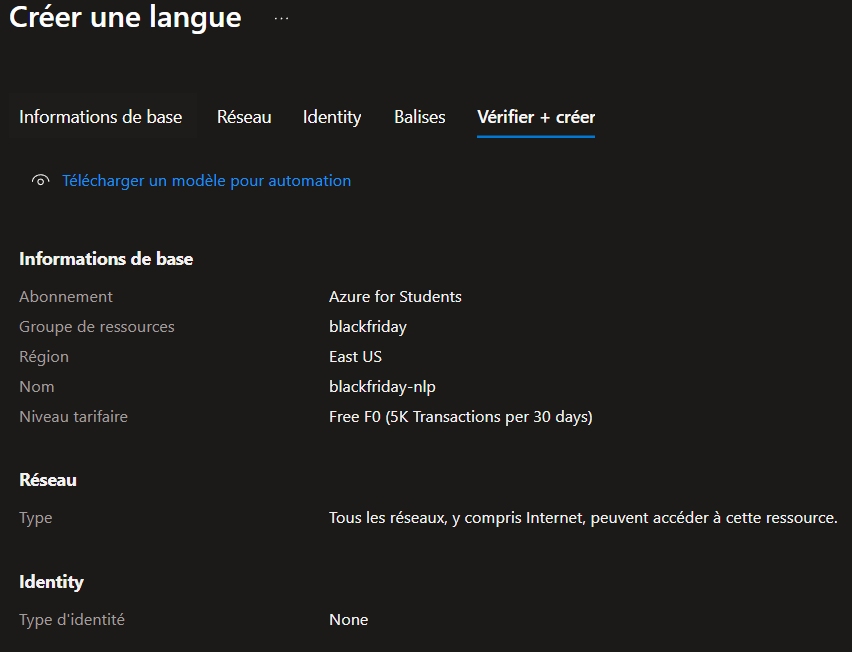
\includegraphics[width=\textwidth]{../pictures/2-azure_ai/2.8-azure_langage2.png}
    \caption{Création du service Language}
  \end{subfigure}
  \hfill
  \begin{subfigure}[b]{0.60\textwidth}
    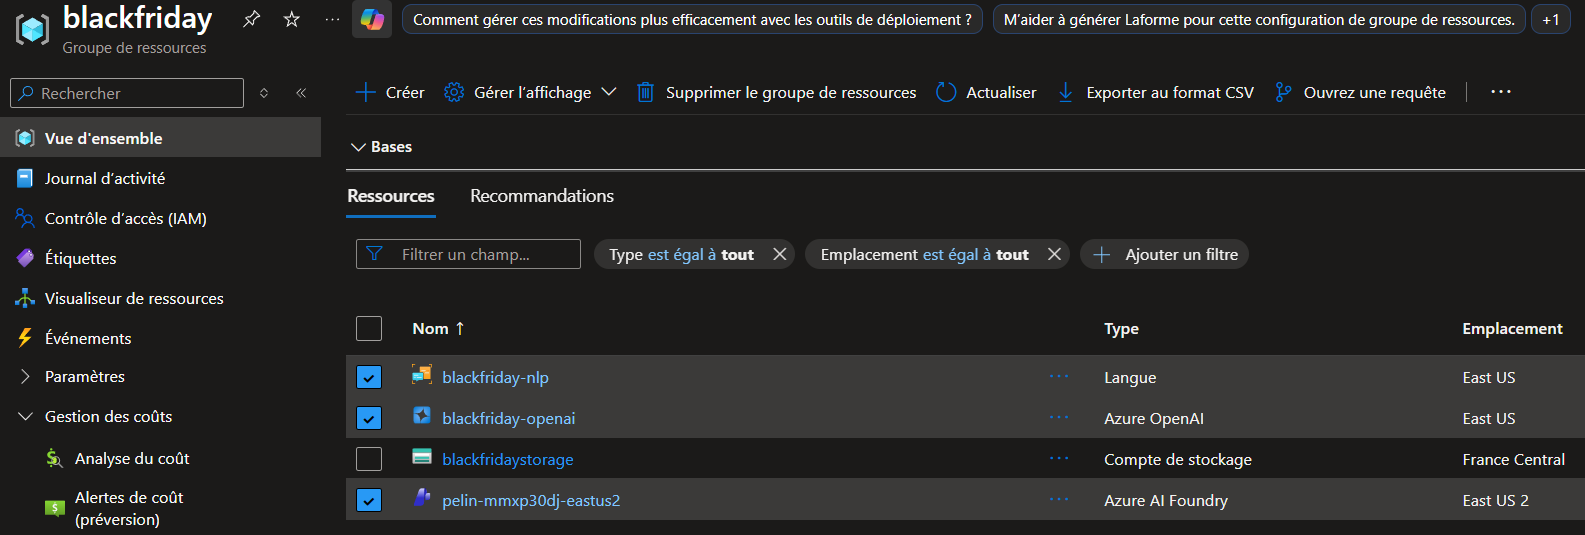
\includegraphics[width=\textwidth]{../pictures/2-azure_ai/2.10-groupe.png}
    \caption{Vue d'ensemble du groupe de ressources}
  \end{subfigure}
  \caption{Azure Text Analytics : configuration et résultats}
\end{figure}

% ──────────────────────────────────────────────────────────────────────────────
\section{Visualisation dans Power BI}

Le dashboard Power BI est connecté directement à \textbf{Azure Blob Storage} (fichiers \mytexttt{blackfriday\_clean.csv}, \mytexttt{reviews\_enriched.csv} et \mytexttt{personas.json}) et structuré en trois pages.

\begin{figure}[H]
  \centering
  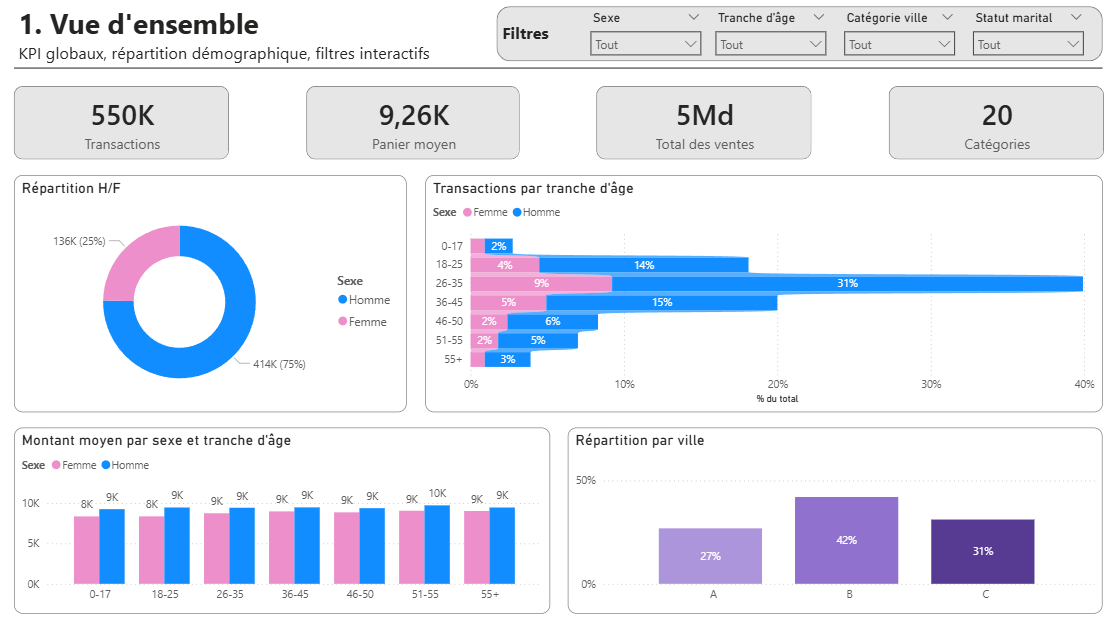
\includegraphics[width=0.7\textwidth]{../pictures/3-power_bi/3.3-page1.png}
  \caption{Page 1. Vue générale : achats par sexe, âge, catégorie de ville}
\end{figure}

\begin{figure}[H]
  \centering
  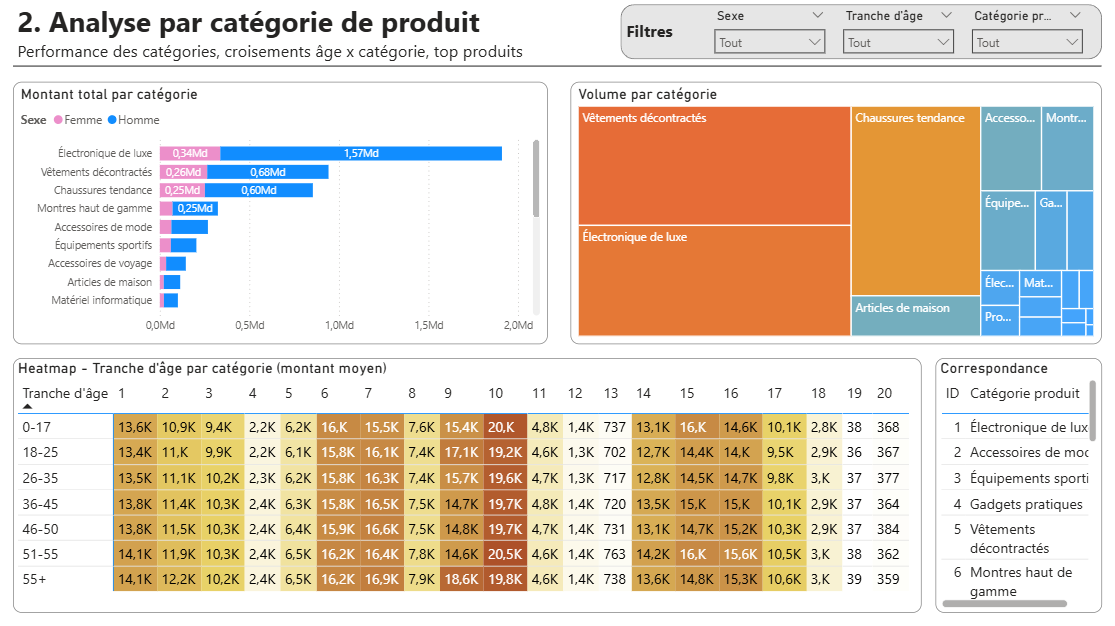
\includegraphics[width=0.7\textwidth]{../pictures/3-power_bi/3.4-page2.png}
  \caption{Page 2. Analyse par catégorie de produits}
\end{figure}

\begin{figure}[H]
  \centering
  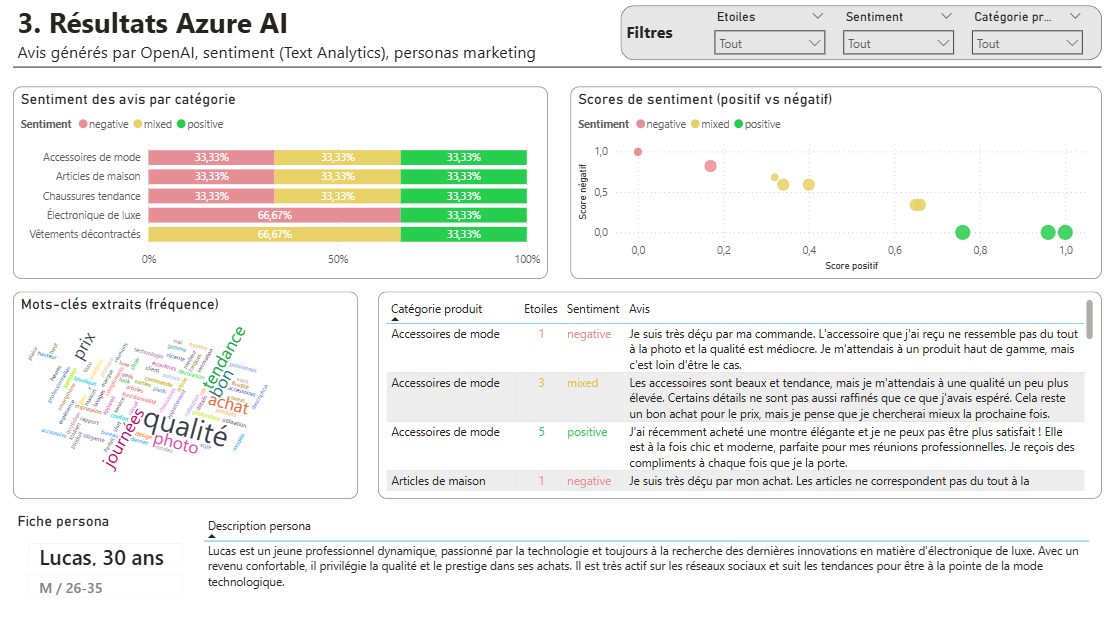
\includegraphics[width=0.7\textwidth]{../pictures/3-power_bi/3.5-page3.png}
  \caption{Page 3. Insights IA : sentiments et mots-clés par catégorie}
\end{figure}

La connexion au Blob Storage permet une \textbf{mise à jour automatique} du rapport dès que les fichiers sources sont modifiés.

% ──────────────────────────────────────────────────────────────────────────────
\section{Observations, découvertes et applications futures}

\subsection{Ce que ce projet m'a appris}

\textbf{Sur Azure :} La prise en main des services Azure est accessible : les API python sont simple d'utilisation et il semble assez aisé de transposer du code, créé pour fonctionner en local, vers le cloud. Toutefois, l'interface du \textbf{portail Azure} est peu intuitive et nécessite une attention particulière à la gestion des ressources et des coûts. Ce dernier point est d'ailleurs assez stressant.
Mais, même en exécutant plusieurs requêtes API vers Azure OpenAI, pour un total de plusieurs milliers de tokens lors des tests, seul \EUR{0.01} de crédit avait été consommé.

\begin{figure}[H]
  \centering
  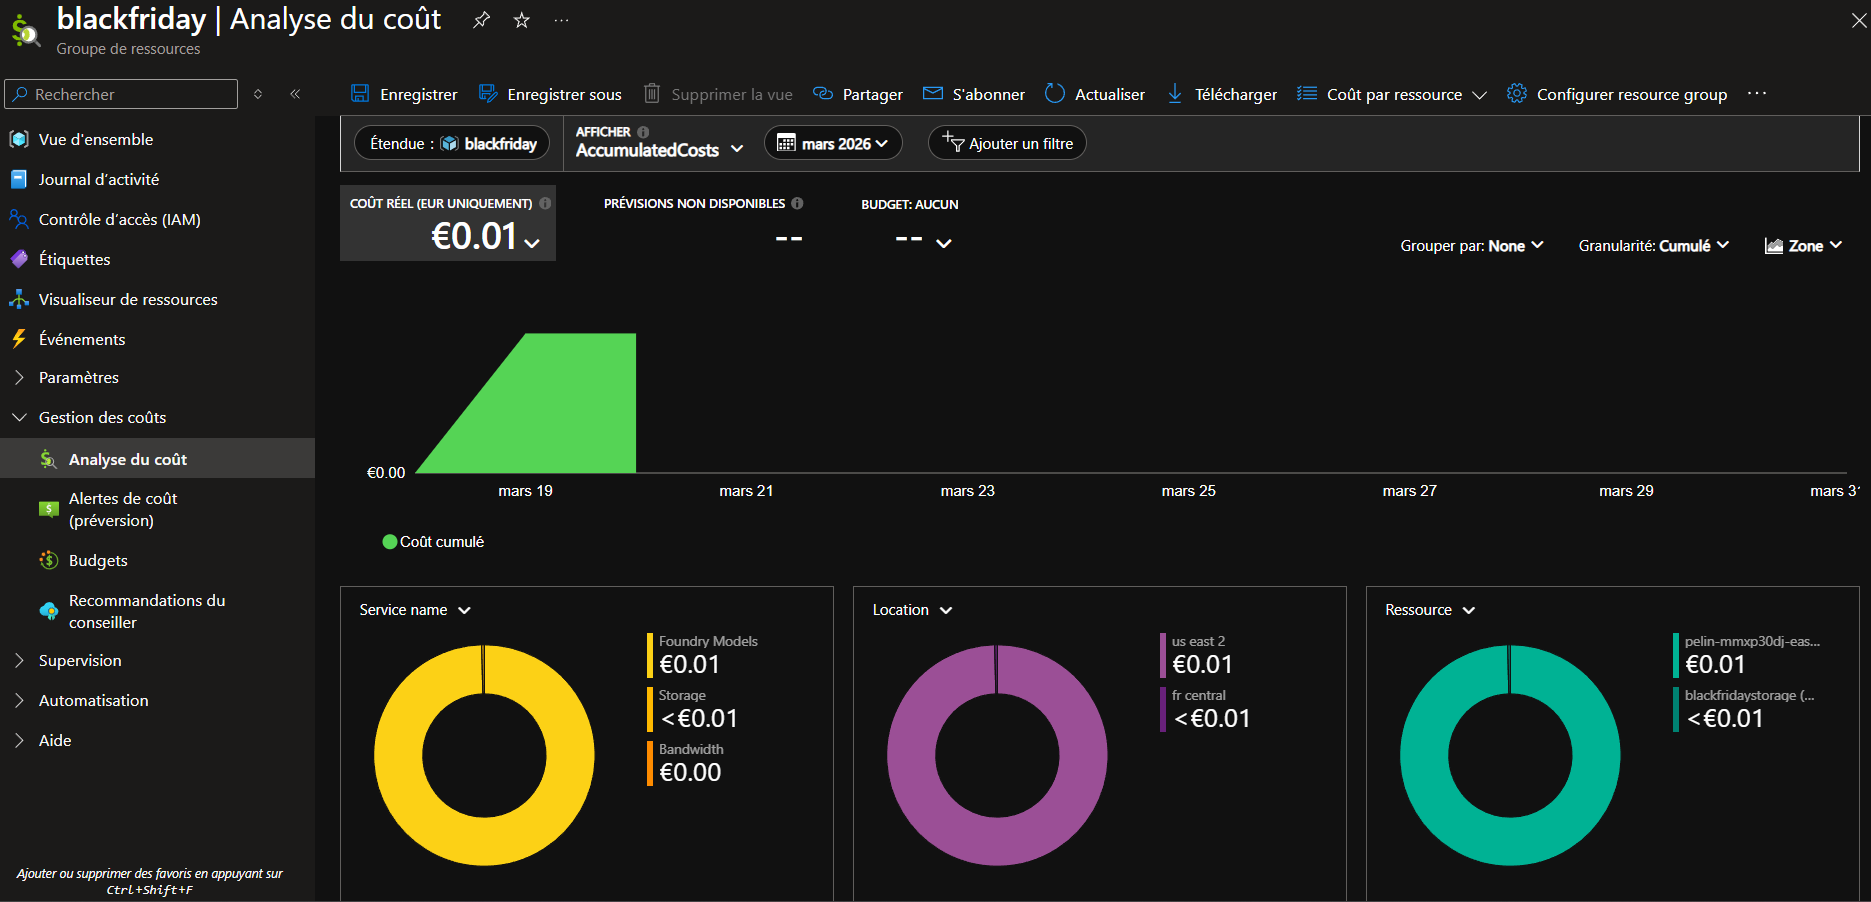
\includegraphics[width=0.8\textwidth]{../pictures/2-azure_ai/2.11-couts.png}
  \caption{Coûts générés par le groupe de ressources à l'issue du projet.}
\end{figure}

\textbf{Sur le coût des API :} Travailler sur des données agrégées (14 segments) plutôt que sur les 550\,068 lignes brutes a sans doute également permis de maîtriser les coûts, tout en obtenant des résultats pertinents. Cela pourrait être une bonne pratique à systématiser avant tout appel LLM en production.

\subsection{Applications professionnelles et futures}

Ce pipeline, même dans sa version simplifiée, préfigure des architectures utilisées en production dans de nombreux contextes :

\begin{description}
  \item[E-commerce \& retail :] Un pipeline similaire (transactions $\to$ Blob $\to$ LLM $\to$ dashboard) permet de générer automatiquement des rapports de veille consommateur, d'alimenter des systèmes de recommandation ou de détecter des tendances d'achat en temps quasi-réel.

  \item[Marketing data-driven :] La génération de personas par LLM à partir de segments RFM est directement applicable : des équipes marketing peuvent disposer de profils narratifs actionnables sans expertise data avancée.

  \item[Analyse de l'e-réputation :] L'analyse de sentiment via Azure Text Analytics est déployable à grande échelle sur de vrais avis clients (Amazon, Trustpilot, réseaux sociaux) pour monitorer la réputation d'une marque ou d'un produit en continu.

  \item[Extension vers du temps réel :] En remplaçant le Blob Storage par \textbf{Azure Event Hubs} et le traitement batch par \textbf{Azure Stream Analytics}, ce pipeline pourrait être adapté à l'analyse de flux d'achats en temps réel (ex. : détection de pic de ventes, alertes fraude).

  \item[MLOps :] Les données enrichies (sentiments, mots-clés, personas) constituent une base pour entraîner des modèles supervisés de recommandation ou de prédiction de churn, déployables via \textbf{Azure Machine Learning}.
\end{description}

D'un point de vue plus personnel, j'envisage d'utiliser Azure pour des petits projets personnels à très faible coûts (si ce n'est gratuit), mais je préfèrerai toujours travailler on-premise.

\subsection{Bilan}

Ce projet a permis de construire un pipeline cloud de bout en bout en mobilisant quatre services Azure complémentaires. Au-delà de la technique, il illustre comment des données brutes, sans valeur textuelle intrinsèque, peuvent être transformées en insights actionnables grâce à l'IA générative et à l'analyse de langue naturelle. Les architectures cloud modernes rendent ces traitements accessibles, scalables et économiquement maîtrisables, à condition de piloter rigoureusement les appels aux services afin de limiter les coûts.

% ──────────────────────────────────────────────────────────────────────────────
\end{document}
